\documentclass[12pt,a4paper]{article}
\usepackage[utf8]{inputenc}
\usepackage{amsmath}
\usepackage{amsfonts}
\usepackage{amssymb}
\usepackage[english]{babel}
\usepackage{tikz}
\usepackage{placeins}
\usepackage{graphicx}
\usepackage{multirow}
\usepackage{hyperref}

\makeatletter
\newcommand*{\rom}[1]{\expandafter\@slowromancap\romannumeral #1@}
\makeatother

\setlength{\parskip}{1ex plus 0.5ex minus 0.2ex}
\newcommand{\hsp}{\hspace{20pt}}
\newcommand{\HRule}{\rule{\linewidth}{0.5mm}}
\newenvironment{remarque}{\textbf{Remarque :}}{}



\title{Présentation des cas d'utilisation principaux}
\author{PaquiTeam}


\begin{document}

\begin{titlepage}
	\begin{center}
	
		
		\vfill
					
		\textsc{\LARGE PaquiTeam}\\[1.5cm]
		
		% Title
		\HRule \\[0.4cm]
			{ \huge \bfseries Présentation des cas d'utilisation principaux :\\
			Paquito, easy packaging\\[0.4cm]
			
\includegraphics[width=0.2\textwidth]{../img/paquito.png}
	
			}
		\HRule \\[1.5cm]
		% Author and supervisor
		
		\begin{minipage}{0.40\textwidth}
			\begin{flushleft} \large
				\emph{Auteurs :}\\
				Lucas \textsc{Robin}\\
				Kevin \textsc{Fleuriot}\\
				Alexandre \textsc{Noiret}\\
				Yassine \textsc{Ait Elmouden}\\
				Seynabou \textsc{Ka}
			\end{flushleft}
		\end{minipage}
		\hfill
		\begin{minipage}{0.40\textwidth}
			\begin{flushright} \large
				\emph{Clients :}\\
				Michael \textsc{Fortier}\\
				Hugues \textsc{Leprieur}
			\end{flushright}
		\end{minipage}

		\vfill			
		{\large 21 janvier 2016}
		\vfill
		\begin{minipage}{0.35\textwidth}
			\begin{flushleft}
				
\includegraphics[width=1\textwidth]{../img/UP13.png}			
			\end{flushleft}
		\end{minipage}
		\hfill
		\begin{minipage}{0.35\textwidth}
			\begin{flushright}
				
\includegraphics[width=1\textwidth]{../img/sup-galile.png}
			\end{flushright}
		\end{minipage}
		
									
	\end{center}		
\end{titlepage}

\section*{Introduction}
	Notre projet se porte sur l'outil Paquito, qui est un outil de génération de paquets pour un logiciel donné. Chaque paquet contient les fichiers de configuration nécessaires pour l'installation et l'utilisation du logiciel. Cet outil est utilisable pour plusieurs distributions de Linux. Le but de notre projet est donc d'améliorer l'utilisation de cet outil. Nous devons premièrement adapter cet outil pour les distributions MacOS. Il faut ensuite développer une interface Web pour faciliter l'utilisation de l'outil Paquito. Enfin nous devons gérer l'exploitation des informations relatives aux paquets (extraction automatique des informations, gestion des dépendances).
	
Dans cet écrit nous allons vous exposer les différents cas d'utilisation de notre système ainsi qu'une première maquette de l'interface Web qui exploitera Paquito.

\section{Diagramme des cas d'utilisation}

	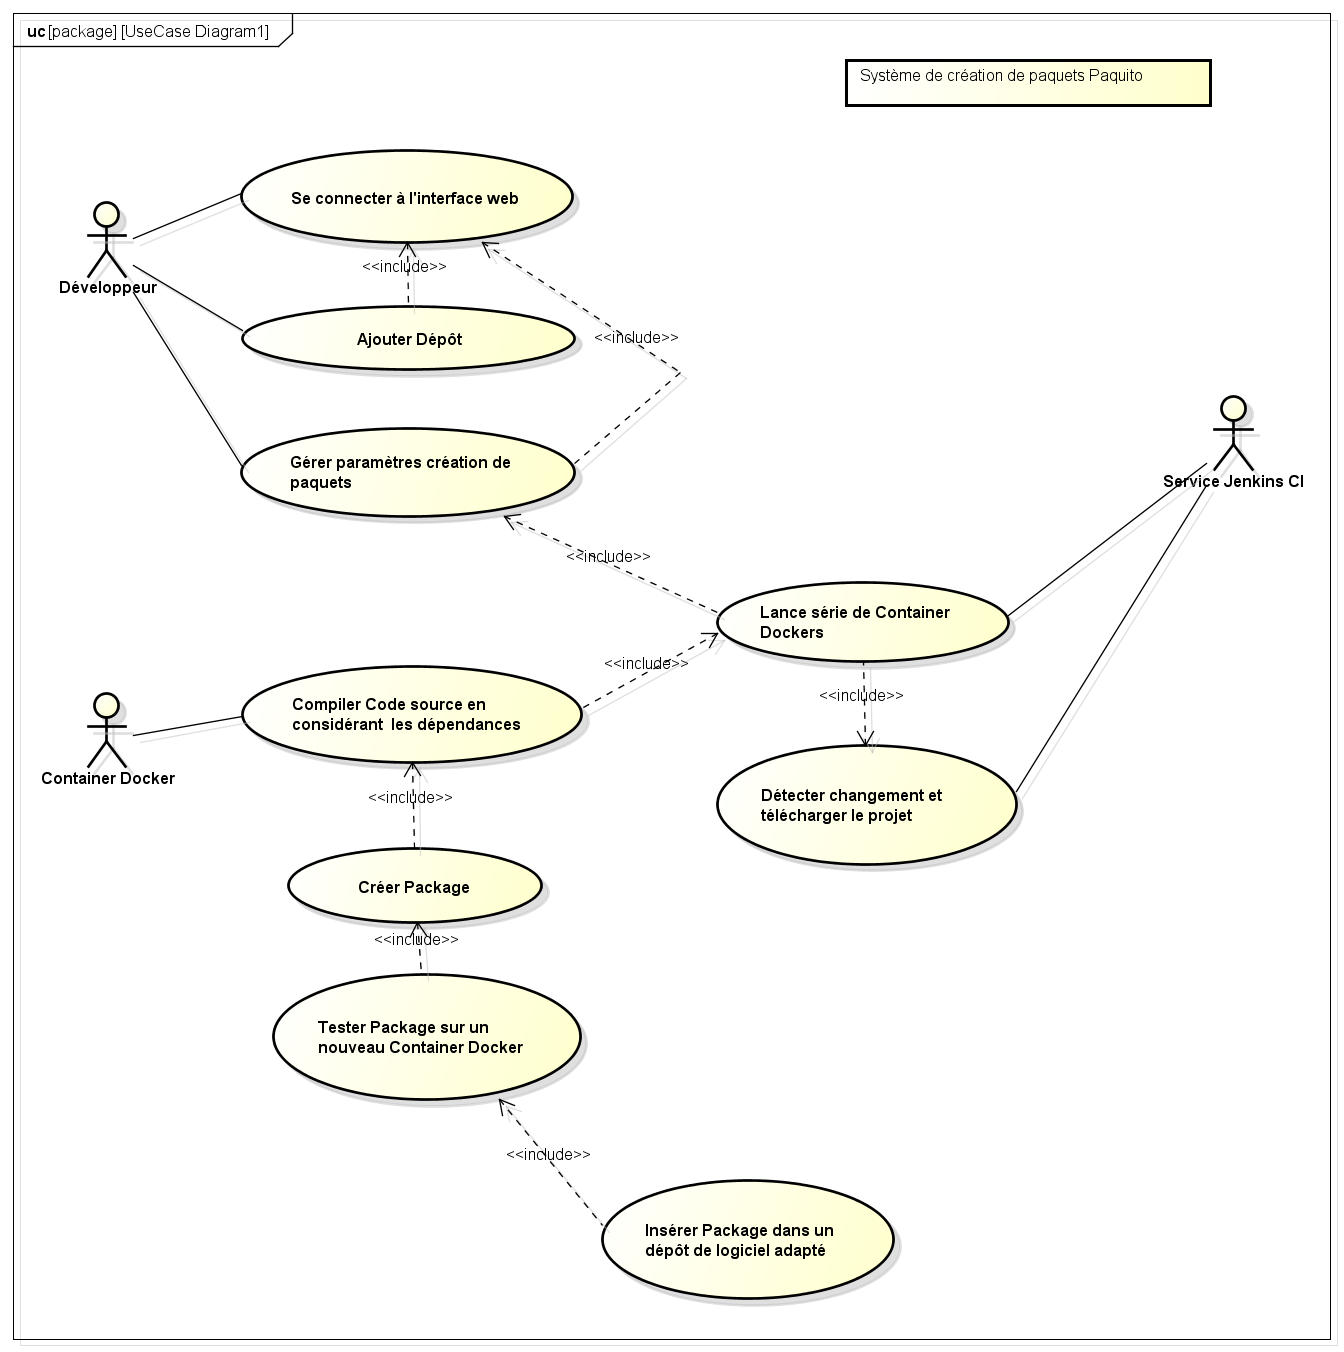
\includegraphics[scale=0.4]{../img/usecasePaquito.png}

\section{Détails des cas d'utilisation}
	\begin{itemize}\renewcommand{\labelitemi}{$\bullet$}
		\item\textbf{ \og Se connecter à l'interface web \fg{}} : Le développeur se connecte à notre interface. 
		\item \textbf{ \og Ajouter dépôt \fg{}} : Il peut télécharger et ajouter un dépôt de son travail.
		\item \textbf{ \og Gérer paramètres de création de paquets \fg{}} : Il peut régler certains paramètres comme la distribution, la version ...
		\item \textbf{ \og Lancer une série de containers Dockers adaptés \fg{}} : Lorsque le développeur ajoute un dépôt, le service Jenkins CI lance une série de containers Dockers adaptés à chaque distribution, ses versions et les architectures.
		\item \textbf{ \og Détecter le changement et télécharger le projet \fg{}} : Le service Jenkins CI détecte un changement et procède au téléchargement du projet. Il récupère par la même occasion un maximum d'informations qui serviront lors de la phase de compilation.
		\item \textbf{ \og Compiler le code source en considérant les dépendances \fg{}} : Le container Docker se charge de compiler le code source à partir des informations récoltées par Jenkins CI 
		\item \textbf{ \og Créer paquetage \fg{}} : Une fois la compilation réussie et le test validé, le système crée le paquetage.
		\item \textbf{ \og Tester le paquetage sur un nouveau container Docker \fg{}}: Le paquetage est testé sur un nouveau container Docker par le système.
		\item \textbf{ \og Insérer paquetage dans un dépôt de logiciel adapté \fg{}} : Une fois que le paquet est réputé conforme et fonctionnel, celui-ci est inséré dans un dépôt de logiciel lié à sa distribution, sa version et son architecture.
	\end{itemize}

\section{Maquette du site}
	Nous avons aussi fait des maquettes de l'interface graphique afin de pouvoir visualiser a quoi elle devra ressembler.

Nous avons dans un premier temps, la maquette de la page de connexion, cela reste classique avec un login et un mot de passe pour s'inscrire et se connecter.
	
	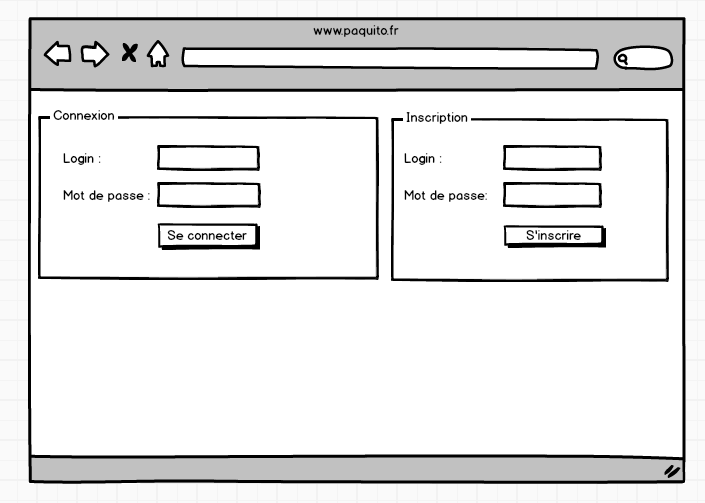
\includegraphics[scale=0.6]{../img/connexionPaquito.png}

Nous avons ensuite l'interface d'ajout de projet à Paquito où il y a un onglet à remplir pour que par la suite Paquito puisse compiler et créer les paquets en fonction de la distribution si une personne voudrait l'installer sur sa machine.

	
	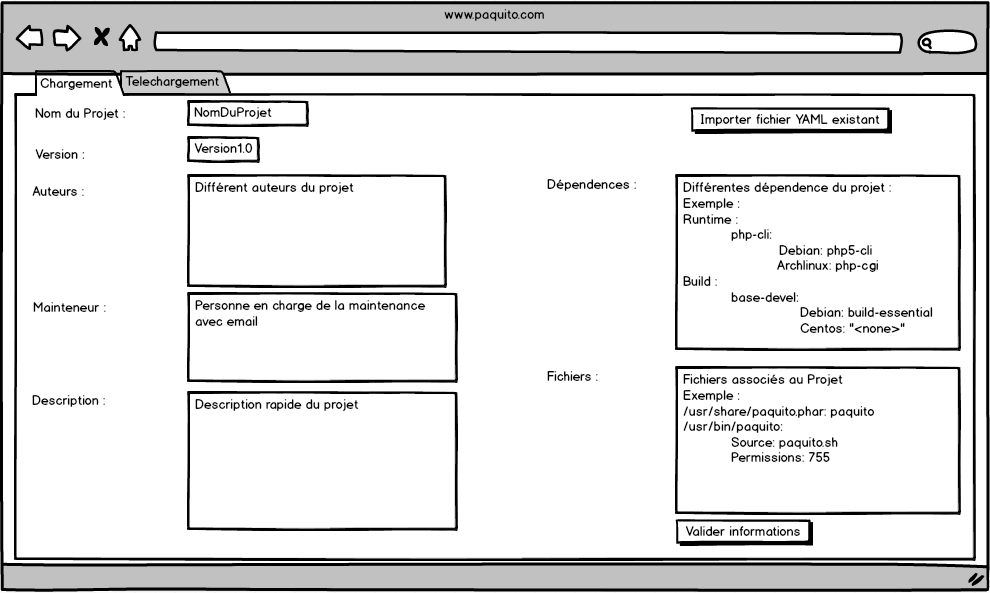
\includegraphics[scale=0.6]{../img/ajouterProjet.png}


Et enfin nous avons la vue d'une page où l'on peut voir des détails sur le projet comme le nom du développeur, le nom du projet.

	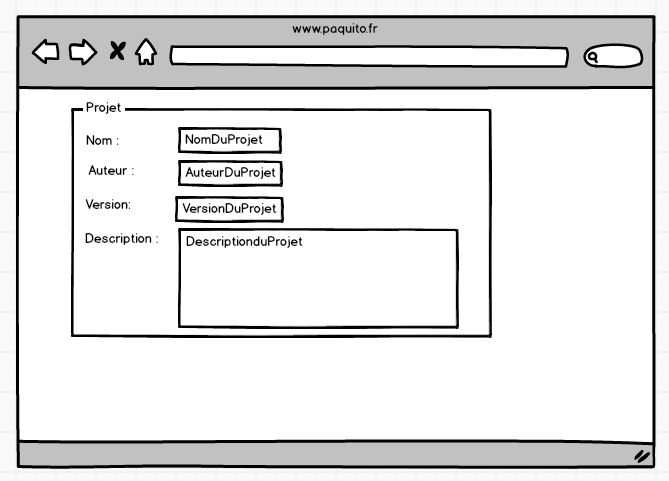
\includegraphics[scale=0.6]{../img/resumeProjet.png}

	
\end{document}
